\chapter{反应的熵与自由能}\label{ch:b2:reaction-free-energy}

运动用冷敷袋内装一袋水和几勺
硝酸铵。挤压冷敷袋，内袋破裂，盐溶解，
几秒钟内袋子便冷到足以缓解扭伤的脚踝。溶解过程
吸收热量——它是\omterm{def:b2:reaction-enthalpy:exothermic}{吸热的}——却仍能自发进行，直至
完成。前一章的焓不能解释全部情况：
反应并不只是“朝放热方向”进行。缺失的量是
熵，物理课中学过的热力学第二定律使其
成为判断一切自发变化的依据。本章列出各物质的熵，
计算反应的熵，并将焓与熵合并为
一个函数，即\omterm{def:b2:reaction-free-energy:gibbs-energy}{吉布斯自由能}，其反应导数决定
恒温恒压下每个反应的方向。

\begin{recall}
由物理学可知：热力学第二定律。每个系统都有一个状态函数，即其
熵 $S$（广延量）；对封闭系统的一个过程，$\dd S =
\delta Q/T_{\text{外}} + \delta S_{\text{c}}$，其中产生的熵
$\delta S_{\text{c}}$ 对可逆变化为零，
否则为正；对组成固定的封闭系统，$\dd U = T\dd S -
p\dd V$。\Cref{ch:b2:reaction-enthalpy}：\omterm{def:b2:reaction-enthalpy:reaction-quantity}{反应量} $\Delta_r X =
(\partial X/\partial\xi)_{T,p}$ 与\omterm{def:b2:reaction-enthalpy:standard-reaction-enthalpy}{标准反应焓}。本科一年级分册
中指出，作为“源自第二定律”的规律，
反应一直进行至 $Q = K^\circ$；本章及后两章将推导
这些规律。
\end{recall}

\begin{omfigure}
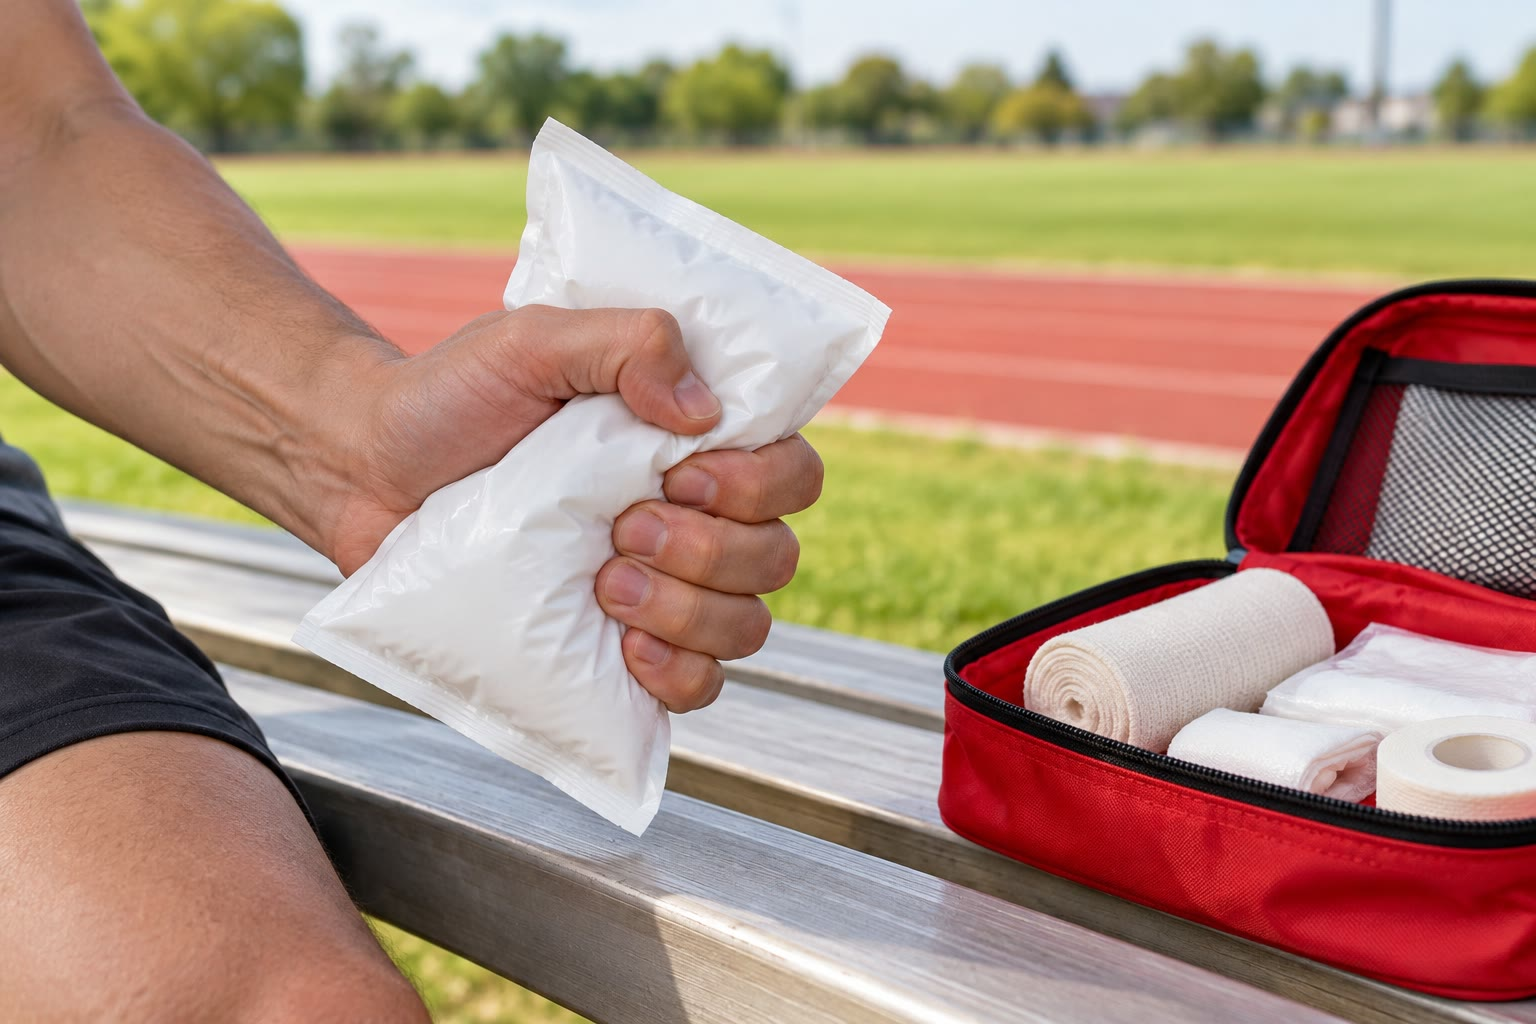
\includegraphics[width=0.55\linewidth]{images/book3/ai/b2-02-cold-pack.jpg}

{\small 冷敷袋：内袋破裂后，硝酸铵
溶于水，袋子随之变冷。该溶解过程吸热且自发，
其熵可解释其原因（见\cref{ex:b2:reaction-free-energy:cold-pack}）。}
\end{omfigure}

\section{标准熵与第三定律}

与焓不同，熵有自然的零点。

\begin{theorem}[热力学第三定律]\label{thm:b2:reaction-free-energy:third-law}
纯净且完全有序的晶体，其熵
随温度趋于 \qty{0}{K} 而趋于零。
\end{theorem}
\admitted

\begin{remark}[零点的来源]\label{rem:b2:reaction-free-energy:third-law}
瓦尔特·能斯特于 1906 年指出，凝聚相之间的\omterm{def:b2:reaction-free-energy:reaction-entropy}{反应熵}在
$T \to 0$ 时趋于零；马克斯·普朗克将其表述为
上述形式。其根源是统计性的：熵计数的是微观
与系统状态相容的排列数，而完美晶体
在 \qty{0}{K} 时只有一种。这一计数在本科三年级分册中
借助配分函数完成。
\end{remark}

\begin{definition}[标准摩尔熵]\label{def:b2:reaction-free-energy:standard-entropy}
称某物质的\emph{标准摩尔熵}\index{标准摩尔熵}
$S^\circ_m(T)$ 为该物质 1 摩尔在
温度 $T$ 下处于标准状态时的熵，其零点即第三定律的零点。
与 $\Delta_f H^\circ$ 不同，它是绝对量，对任何物质都为正，
单质也不例外。
\end{definition}

\begin{proposition}[由热容求绝对熵]\label{prop:b2:reaction-free-energy:absolute-entropy}
在恒压 $p^\circ$ 下将物质从 \qty{0}{K} 加热到 $T$，
\[
  S^\circ_m(T) = \int_0^T\frac{C^\circ_{p,m}(T')}{T'}\,\dd T' +
  \sum_{\text{相变}}\frac{\Delta_{\text{trs}}H^\circ}{T_{\text{trs}}} ,
\]
其中积分在每个相内按其温度范围进行。
\end{proposition}

\begin{proof}
对物质恒压可逆加热：$\delta S_{\text{c}} =
0$，$\delta Q = \dd H = C_p\,\dd T$，故 $\dd S = C_p\,\dd T/T$。在
相变（熔化、沸腾）处，温度保持为 $T_{\text{trs}}$，
而热量 $\Delta_{\text{trs}}H$ 是可逆吸收的，熵
跃变 $\Delta_{\text{trs}}H/T_{\text{trs}}$。再将自
第三定律零点起算的各部分相加。
\end{proof}

\begin{omfigure}
\begin{tikzpicture}
\begin{axis}[
  width=0.8\linewidth, height=6.2cm, xmin=0, xmax=1500, ymin=0, ymax=210,
  axis x line=bottom, axis y line=left, xlabel={温度 $T$（K）},
  ylabel={锌的 $S^\circ_m$（\unit{J/(K.mol)}）},
  xtick={0,250,500,750,1000,1250,1500},
  tick label style={font=\small}, label style={font=\small}, clip=false]
\addplot[omDef, very thick, smooth] table[x=T, y=S] {figdata/out/bachelor-2-standard-entropy-solid.dat};
\addplot[omProp, very thick] table[x=T, y=S] {figdata/out/bachelor-2-standard-entropy-liquid.dat};
\addplot[omThm, very thick] table[x=T, y=S] {figdata/out/bachelor-2-standard-entropy-gas.dat};
\draw[densely dashed, gray] (axis cs:692.73,64.6) -- (axis cs:692.73,75.2);
\draw[densely dashed, gray] (axis cs:1180.2,91.9) -- (axis cs:1180.2,189.6);
\node[omDef, font=\small, anchor=south east] at (axis cs:600,60) {固体};
\node[omProp, font=\small, anchor=north west] at (axis cs:850,78) {液体};
\node[omThm, font=\small, anchor=south] at (axis cs:1350,192) {气体};
\node[font=\scriptsize, anchor=west, align=left] at (axis cs:700,110) {熔化，$+10.6$\\ 在 \qty{692.7}{K}};
\node[font=\scriptsize, anchor=east, align=right] at (axis cs:1170,150) {沸腾，\\ $+97.7$ 在 \\ \qty{1180.2}{K}};
\end{axis}
\end{tikzpicture}

{\small 锌的\omterm{def:b2:reaction-free-energy:standard-entropy}{标准摩尔熵}，零点取自第三定律。它随温度升高而增大，
因为金属储存热量；在熔点处熵按
$\Delta_{\text{fus}}H/T_{\text{fus}}$ 跃升，在沸点处跃升更大，
按 $\Delta_{\text{vap}}H/T_b$：气体远比
液体无序。}
% ledger: s0T:Zn_crl.0, s0T:Zn_crl.298.15, s0T:Zn_cr.692, s0T:Zn_l.692, s0T:Zn_l.1180, s0T:Zn_g.1180, hT:Zn_cr.692, hT:Zn_l.692, hT:Zn_l.1180, hT:Zn_g.1180, dfh:Zn_g (curve in figdata/bachelor-2/standard-entropy.py)
\end{omfigure}

图中给出了值得记住的数量级。在室温下，
金属或硬质晶体的熵约为几十
\unit{J/(K.mol)}，液体约为一百，气体为一至三百；
熔化时增加不多，沸腾时增加很多。本册所用的\omterm{def:b2:reaction-free-energy:standard-entropy}{标准摩尔熵}
与生成焓一并列于表中。

\section{反应熵}

\begin{definition}[反应熵]\label{def:b2:reaction-free-energy:reaction-entropy}
称\emph{反应熵}\index{反应熵}为 $\Delta_r S =
(\partial S/\partial\xi)_{T,p}$，称\emph{标准反应
熵}\index{标准反应熵}为 $\Delta_r S^\circ(T) =
\sum_i\nu_iS^\circ_{m,i}(T)$，单位为 \unit{J/(K.mol)}。
\end{definition}

因为标准熵是绝对的，所以无需生成反应：
参与反应的单质按其自身的熵计入。

\begin{example}[三个反应熵]\label{ex:b2:reaction-free-energy:entropies}
在 \qty{298.15}{K} 下：
\begin{itemize}
  \item \ce{CaCO3(s) -> CaO(s) + CO2(g)}: $\Delta_r S^\circ = 39.75 + 213.79 -
        92.9 = \qty{+160.6}{J/(K.mol)}$，由固体生成气体；
  \item \ce{N2(g) + 3H2(g) -> 2NH3(g)}: $\Delta_r S^\circ = 2(192.77) -
        191.61 - 3(130.68) = \qty{-198.1}{J/(K.mol)}$，四个气体分子
        变为两个；
  \item \ce{N2O4(g) -> 2NO2(g)}: $\Delta_r S^\circ = 2(240.03) - 304.38 =
        \qty{+175.7}{J/(K.mol)}$.
\end{itemize}
% ledger: s0:CaCO3_cr, s0:CaO_cr, s0:CO2_g, s0:N2_g, s0:H2_g, s0:NH3_g, s0:N2O4_g, s0:NO2_g (computed in figdata/bachelor-2/thermo-data.py)
\end{example}

\begin{proposition}[反应熵的符号]\label{prop:b2:reaction-free-energy:sign-rule}
当有气体参与时，$\Delta_r S^\circ$ 的符号一般与
$\Delta\nu_{\text{气体}} = \sum_{\text{气体}}\nu_i$ 的符号相同，其大小约为
\qty{100}{} 至 \qty{200}{J/(K.mol)}，每生成或消耗一摩尔气体。当
$\Delta\nu_{\text{气体}} = 0$，或不涉及气体时，$\Delta_r S^\circ$ 很
小，其符号必须计算。
\end{proposition}

\begin{proof}[论证]
气体在 \qty{298}{K} 下的摩尔熵介于 130 与
\qty{300}{J/(K.mol)} 之间，固体或液体的摩尔熵仅为几十：生成或
消耗一摩尔气体的贡献压过其他一切贡献。这只是一条
经验法则，而非定理：盐的溶解过程不涉及气体，却仍可
使熵改变一百 \unit{J/(K.mol)}。
\end{proof}

\begin{method}[判断 $\Delta_r S^\circ$ 的符号]\label{met:b2:reaction-free-energy:entropy-sign}
\begin{enumerate}
  \item 计算 $\Delta\nu_{\text{气体}}$：若其不为零，则由它决定
        符号。
  \item 否则比较各状态的有序程度：溶解晶体、
        熔化、将一个分子拆成两部分都会使熵增大；
        沉淀、凝固、将两个分子结合为一个都会使熵减小。
  \item 需要做出判断时，计算 $\sum_i\nu_iS^\circ_{m,i}$。
\end{enumerate}
\end{method}

本科一年级分册中提到过一个结论：消除反应
在相同试剂下生成的分子比取代反应更多（烯烃、离去基团
与质子化的碱，对比取代生成物与离去
基团）。其\omterm{def:b2:reaction-free-energy:reaction-entropy}{反应熵}更大，熵项随温度升高而增大
（见下一节），这正是加热有利于
消除而不利于取代的原因。

\section{吉布斯自由能}

\begin{definition}[吉布斯自由能]\label{def:b2:reaction-free-energy:gibbs-energy}
称系统的\emph{吉布斯自由能}\index{吉布斯自由能}（或称吉布斯自由能）
为状态函数 $G = H - TS$，是广延量，单位为焦耳。
\end{definition}

\begin{definition}[反应吉布斯自由能]\label{def:b2:reaction-free-energy:reaction-gibbs}
称\emph{反应吉布斯自由能}\index{反应吉布斯自由能}为 $\Delta_r G
= (\partial G/\partial\xi)_{T,p}$，称\emph{标准反应吉布斯
自由能}\index{标准反应吉布斯自由能}为 $\Delta_r G^\circ(T) =
\sum_i\nu_iG^\circ_{m,i}(T)$，两者单位均为 \unit{kJ/mol}。
\end{definition}

\begin{proposition}[焓项与熵项]\label{prop:b2:reaction-free-energy:g-h-s}
$\Delta_r G = \Delta_r H - T\Delta_r S$，且 $\Delta_r G^\circ = \Delta_r
H^\circ - T\Delta_r S^\circ$.
\end{proposition}

\begin{proof}
对 $G = H - TS$ 关于 $\xi$ 在 $T$、$p$ 固定时求导：$T$
是求导中的常数。
\end{proof}

\begin{proposition}[反应系统中 $G$ 的微分]\label{prop:b2:reaction-free-energy:dG}
对于一个封闭系统，其中发生一个反应，温度 $T$ 与
压强 $p$ 均匀，
\[
  \dd G = V\,\dd p - S\,\dd T + \Delta_r G\,\dd\xi .
\]
\end{proposition}

\begin{proof}
$G(T, p, \xi)$ 的全微分为 $\dd G = (\partial G/\partial
T)_{p,\xi}\dd T + (\partial G/\partial p)_{T,\xi}\dd p + \Delta_r G\,\dd\xi$.
前两个偏导数在组成固定时取值：它们即为
组成固定的封闭系统的偏导数，由物理学可得
$\dd U = T\dd S - p\dd V$，于是 $\dd G = \dd U + p\dd V + V\dd p - T\dd S
- S\dd T = V\dd p - S\dd T$。因此 $(\partial G/\partial T)_{p,\xi} = -S$
且 $(\partial G/\partial p)_{T,\xi} = V$。
\end{proof}

\section{演化判据}

\begin{theorem}[演化判据]\label{thm:b2:reaction-free-energy:evolution}
在恒温恒压的封闭系统中，不交换
除压力所做功以外的功，反应只能朝
使下式成立的方向进行：
\[
  \Delta_r G\,\dd\xi \leq 0 ,
\]
等号在平衡时成立。若 $\Delta_r G < 0$，反应正向进行，
若 $\Delta_r G > 0$，反应逆向进行，系统
当 $\Delta_r G = 0$ 时处于平衡状态。
\end{theorem}

\begin{proof}
在均匀的 $T$ 和 $p$ 下取一无穷小变化，二者
与外界的相同。仅计压强功时，第一定律只给出 $\dd U = \delta Q
- p\dd V$；第二定律给出 $\delta Q = T\dd S - T\delta S_{\text{c}}$。于是
\[
  \dd G = \dd U + p\dd V + V\dd p - T\dd S - S\dd T = -T\,\delta
  S_{\text{c}} + V\dd p - S\dd T .
\]
与\cref{prop:b2:reaction-free-energy:dG}比较，在 $T$ 和 $p$ 固定时：
$\Delta_r G\,\dd\xi = -T\,\delta S_{\text{c}}$。由于 $\delta S_{\text{c}}
\geq 0$，故 $\Delta_r G\,\dd\xi \leq 0$；$\delta S_{\text{c}} = 0$（一个
可逆的平衡变化）要求 $\Delta_r G = 0$。
\end{proof}

\begin{remark}[判据说明了什么，又不说明什么]\label{rem:b2:reaction-free-energy:criterion}
在 $T$ 和 $p$ 恒定时，反应产生的熵为 $-\Delta_r G\,
\dd\xi/T$。\omterm{def:b2:reaction-free-energy:gibbs-energy}{吉布斯自由能}即第二定律限于实验室条件时的形式，
且只用系统自身的量写出。它说明
反应可以朝哪个方向进行，从不说明进行得多快：金刚石，
其转化为石墨的 $\Delta_r G^\circ < 0$，却能在戒指上
永远保持不变。它还假定没有其他功：产生电功的电池，或接收电功的电解槽，
服从修正后的判据
（见\cref{ch:b2:cell-thermodynamics}）。
\end{remark}

\begin{definition}[放能与吸能]\label{def:b2:reaction-free-energy:exergonic}
在给定状态下，反应称为\emph{放能的}\index{放能的}，条件是
$\Delta_r G < 0$；称为\emph{吸能的}\index{吸能的}，条件是 $\Delta_r G >
0$。所有物种均处于标准态时，这些术语适用于
$\Delta_r G^\circ$ 的符号。
\end{definition}

判据用的是 $\Delta_r G$，即系统在实际状态下的值，
$\Delta_r G^\circ$ 指所有物种均处于标准态时的值，
这在实际混合物中很少出现。二者之间通过组成相联系，
这是\cref{ch:b2:chemical-potential}的内容，并在
\cref{ch:b2:equilibrium-shifts}中给出本科一年级的定律 $Q = K^\circ$。对于
纯固体与纯液体之间的反应，以及 \qty{1}{bar} 下的气体反应，
两者相同。

\begin{example}[冷敷袋]\label{ex:b2:reaction-free-energy:cold-pack}
对于 \ce{NH4NO3(s) -> NH4+(aq) + NO3-(aq)}，在 \qty{298.15}{K} 下，取标准态：
$\Delta_r H^\circ = -339.87 + 365.56 = \qty{+25.69}{kJ/mol}$ 和
$\Delta_r S^\circ = 259.8 - 151.08 = \qty{+108.7}{J/(K.mol)}$，于是
$\Delta_r G^\circ = 25.69 - 298.15 \times 0.1087 = \qty{-6.7}{kJ/mol}$：
溶解过程吸热且放能。水中自由运动的离子比
在晶体中更加无序，熵项 $T\Delta_r
S^\circ = \qty{32.4}{kJ/mol}$ 超过了焓的代价。
% ledger: dfh:NH4NO3_cr, s0:NH4NO3_cr, dfh:NH4NO3_ai, s0:NH4NO3_ai (computed in figdata/bachelor-2/thermo-data.py)
\end{example}

\begin{history}[约西亚·威拉德·吉布斯]
\begin{minipage}[t]{0.2\linewidth}\vspace{0pt}
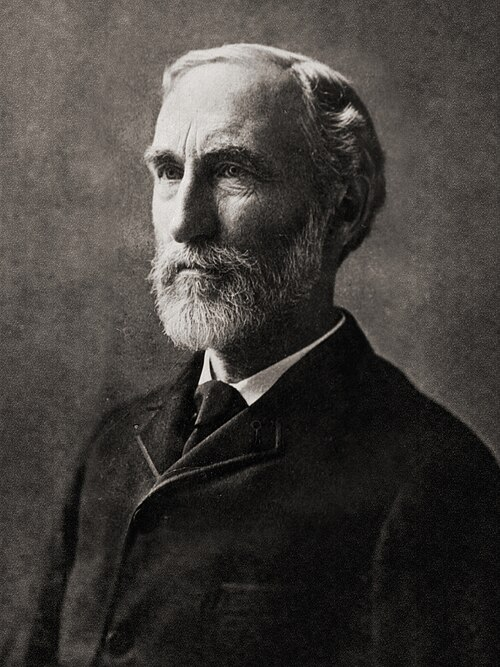
\includegraphics[width=\linewidth]{images/book3/gibbs.jpg}
\end{minipage}\hfill
\begin{minipage}[t]{0.76\linewidth}\vspace{0pt}
约西亚·威拉德·吉布斯（1839--1903），耶鲁大学的数学物理教授，
于 1876 年至 1878 年间发表了《论非均相物质的平衡》
，约三百页，刊于一家小型学会的会刊，
其中包含了自由能、化学势以及后续各章将出现的
相律。很少有化学家读过它，直到
1890 年代才有译本。（照片：公有领域，维基共享资源
）。
\end{minipage}
\end{history}

\section{标准反应吉布斯自由能与温度}

\begin{definition}[埃林厄姆近似]\label{def:b2:reaction-free-energy:ellingham-approximation}
\emph{埃林厄姆近似}\index{埃林厄姆近似}认为
$\Delta_r H^\circ$ 与 $\Delta_r S^\circ$ 视为与温度无关，
在不含相变的温度区间内。于是 $\Delta_r G^\circ(T)
= \Delta_r H^\circ - T\Delta_r S^\circ$ 是关于 $T$ 的直线，斜率为
$-\Delta_r S^\circ$。
\end{definition}

\begin{proposition}[温度导数]\label{prop:b2:reaction-free-energy:gibbs-helmholtz}
\[
  \frac{\dd\Delta_r G^\circ}{\dd T} = -\Delta_r S^\circ, \qquad
  \frac{\dd}{\dd T}\!\left(\frac{\Delta_r G^\circ}{T}\right) =
  -\frac{\Delta_r H^\circ}{T^2}\ \ \text{（吉布斯–亥姆霍兹）}, \qquad
  \frac{\dd\Delta_r S^\circ}{\dd T} = \frac{\Delta_r C^\circ_p}{T}.
\]
特别地，当 $\Delta_r C^\circ_p$
较小时，\omterm{def:b2:reaction-free-energy:ellingham-approximation}{埃林厄姆近似}成立。
\end{proposition}

\begin{proof}
所有物种均处于标准态时，$G^\circ(T, \xi)$ 有 $(\partial
G^\circ/\partial T)_\xi = -S^\circ$（见\cref{prop:b2:reaction-free-energy:dG}）。
由施瓦茨定理，
\[
  \frac{\dd\Delta_r G^\circ}{\dd T} = \partial_\xi\partial_T G^\circ =
  -\partial_\xi S^\circ = -\Delta_r S^\circ .
\] 于是 $\frac{\dd}{\dd
T}(\Delta_r G^\circ/T) = \frac{-T\Delta_r S^\circ - \Delta_r G^\circ}{T^2} =
-\frac{\Delta_r H^\circ}{T^2}$。最后，$\dd S^\circ_m = C^\circ_{p,m}\,\dd
T/T$ 对每种物种成立（见\cref{prop:b2:reaction-free-energy:absolute-entropy}），
并由同样的组合得到最后一个关系式。若 $\Delta_r C^\circ_p$
较小，$\Delta_r H^\circ$（基尔霍夫）与 $\Delta_r S^\circ$ 几乎不变。
\end{proof}

\begin{definition}[转变温度]\label{def:b2:reaction-free-energy:inversion-temperature}
当 $\Delta_r H^\circ$ 与 $\Delta_r S^\circ$ 同号时，
反应的\emph{转变温度}\index{转变温度}是使
$\Delta_r G^\circ$ 改变符号的温度；在\omterm{def:b2:reaction-free-energy:ellingham-approximation}{埃林厄姆近似}下，
$T_i = \Delta_r H^\circ/\Delta_r S^\circ$。
\end{definition}

\begin{omfigure}
\begin{tikzpicture}
\begin{axis}[
  width=0.72\linewidth, height=5.6cm, xmin=0, xmax=1600, ymin=0, ymax=260,
  axis x line=bottom, axis y line=left, xlabel={$T$ (K)}, ylabel={\unit{kJ/mol}},
  tick label style={font=\small}, label style={font=\small}, clip=false]
\addplot[omThm, very thick] table[x=T, y=DrH] {figdata/out/bachelor-2-thermo-data-calcite.dat};
\addplot[omDef, very thick] table[x=T, y=TDrS] {figdata/out/bachelor-2-thermo-data-calcite.dat};
\node[omThm, anchor=south west, font=\small] at (axis cs:60,180) {$\Delta_r H^\circ = 178.3$};
\node[omDef, anchor=west, font=\small] at (axis cs:1600,257) {$T\Delta_r S^\circ$};
\draw[dotted] (axis cs:1110,0) -- (axis cs:1110,178.3);
\node[anchor=south west, font=\small] at (axis cs:1120,8) {$T_i = \qty{1110}{K}$};
\node[font=\scriptsize, align=center] at (axis cs:600,140) {$\Delta_r G^\circ > 0$：\\ 方解石稳定};
\node[font=\scriptsize, align=center] at (axis cs:1470,206) {$\Delta_r G^\circ < 0$};
\end{axis}
\end{tikzpicture}

{\small \omterm{def:b2:reaction-free-energy:ellingham-approximation}{埃林厄姆近似}下，反应 \ce{CaCO3(s) -> CaO(s) + CO2(g)} 的焓项与熵项。
低于\omterm{def:b2:reaction-free-energy:inversion-temperature}{转变温度}时，
焓的代价占优，石灰石在 \qty{1}{bar} 的二氧化碳分压下稳定；
高于\omterm{def:b2:reaction-free-energy:inversion-temperature}{转变温度}时，熵项占优，石灰石分解。}
% ledger: dfh:CaCO3_cr, dfh:CaO_cr, dfh:CO2, s0:CaCO3_cr, s0:CaO_cr, s0:CO2_g (computed in figdata/bachelor-2/thermo-data.py)
\end{omfigure}

\begin{omfigure}
\begin{tikzpicture}[font=\small]
  \draw[thick] (0,0) rectangle (8,4);
  \draw[thick] (4,0) -- (4,4) (0,2) -- (8,2);
  \node[above] at (2,4) {$\Delta_r H^\circ < 0$};
  \node[above] at (6,4) {$\Delta_r H^\circ > 0$};
  \node[left] at (0,3) {$\Delta_r S^\circ > 0$};
  \node[left] at (0,1) {$\Delta_r S^\circ < 0$};
  \node[align=center, omDef] at (2,3) {放能的 \\ 任意 $T$};
  \node[align=center, omProp] at (6,3) {放能的 \\ 高于 $T_i$};
  \node[align=center, omProp] at (2,1) {放能的 \\ 低于 $T_i$};
  \node[align=center, omThm] at (6,1) {吸能的 \\ 任意 $T$};
\end{tikzpicture}

{\small \omterm{def:b2:reaction-free-energy:ellingham-approximation}{埃林厄姆近似}下，$\Delta_r G^\circ = \Delta_r H^\circ - T\Delta_r
S^\circ$ 的四种情形：燃烧位于左上方框内；
石灰石的分解与冷敷袋位于右上方框内；
氨的合成位于左下方框内。}
\end{omfigure}

\begin{method}[温度 $T$ 下的标准反应吉布斯自由能]\label{met:b2:reaction-free-energy:delta-g-standard}
\begin{enumerate}
  \item 由 \qty{298.15}{K} 时的数据表，计算 $\Delta_r H^\circ$ 和
        $\Delta_r S^\circ$.
  \item 检查 \qty{298}{K} 至 $T$ 之间没有物质改变状态；
        否则计入相变（焓与熵）的贡献，或
        从新状态出发。
  \item \omterm{def:b2:reaction-free-energy:ellingham-approximation}{埃林厄姆近似}下，$\Delta_r G^\circ(T) = \Delta_r H^\circ
        - T\Delta_r S^\circ$.
  \item 若 $\Delta_r C^\circ_p$ 不小或区间较长，
        则直接使用表中给出的 $\Delta_f G^\circ(T)$。
\end{enumerate}
\end{method}

\begin{example}[近似的两项检验]\label{ex:b2:reaction-free-energy:tests}
对于石灰石，$\Delta_r C^\circ_p = 42.80 + 37.13 - 81.88 =
\qty{-2.0}{J/(K.mol)}$：近似效果极好，且 $\Delta_r
G^\circ = 178.3 - T \times 0.1606$ 给出 $T_i = \qty{1110}{K}$。对于氨，
$\Delta_r G^\circ(700) \approx -91.9 + 700 \times 0.1981 =
\qty{+46.8}{kJ/mol}$，而表中给出 $2\Delta_f G^\circ(\ce{NH3}, 700) =
\qty{+54.4}{kJ/mol}$：此处 $\Delta_r C^\circ_p = \qty{-44}{J/(K.mol)}$，而
误差为 \qty{8}{kJ/mol}，使该温度下的平衡常数相差
4 倍。
% ledger: cp:CaO_cr.298, cp:CO2_g.298, cp:CaCO3_cr.298, janafG:NH3.700 (computed in figdata/bachelor-2/thermo-data.py)
\end{example}

\section{练习}

\begin{exercise}[$\star$]\label{exo:b2:reaction-free-energy:1}
预测下列反应的 $\Delta_r S^\circ$ 的符号：(a) \ce{2H2(g) + O2(g) -> 2H2O(l)}；
(b) \ce{CaCO3(s) -> CaO(s) + CO2(g)}；(c) \ce{N2O4(g) -> 2NO2(g)}；
(d) \ce{Ag+(aq) + Cl-(aq) -> AgCl(s)}；(e) \ce{H2O(s) -> H2O(l)}；
(f) \ce{H2(g) + Cl2(g) -> 2HCl(g)}。
\end{exercise}

\begin{exercise}[$\star$]\label{exo:b2:reaction-free-energy:2}
计算 \qty{298.15}{K} 时的 $\Delta_r S^\circ$ 与 $\Delta_r G^\circ$，
氨合成反应 \ce{N2(g) + 3H2(g) -> 2NH3(g)}，已知 $\Delta_r
H^\circ = \qty{-91.9}{kJ/mol}$ 及本章中的熵值。
该反应是否放能？
\end{exercise}

\begin{exercise}[$\star$]\label{exo:b2:reaction-free-energy:3}
计算 $\Delta_r G^\circ(\qty{298.15}{K})$，反应 \ce{H2(g) + 1/2O2(g) ->
H2O(l)} 由 $\Delta_f H^\circ(\ce{H2O}, \text{l}) = \qty{-285.83}{kJ/mol}$
及标准熵 \ce{H2(g)} 130.68，\ce{O2(g)} 205.15，
\ce{H2O(l)} \qty{69.95}{J/(K.mol)}。为何该数值是液态水的
标准生成\omterm{def:b2:reaction-free-energy:gibbs-energy}{吉布斯自由能}？
% ledger: dfh:H2O-l, s0:H2_g, s0:O2_g, s0:H2O_l
\end{exercise}

\begin{exercise}[$\star$]\label{exo:b2:reaction-free-energy:4}
利用锌的熵图，读出其在
\qty{298}{K} 与 \qty{1000}{K} 时的\omterm{def:b2:reaction-free-energy:standard-entropy}{标准摩尔熵}，以及在熔点与沸点处的跃变，
并由此推出熔化焓与汽化焓。
\end{exercise}

\begin{exercise}[$\star\star$]\label{exo:b2:reaction-free-energy:5}
对于 \ce{H2O(l) -> H2O(g)}，在 \qty{298.15}{K} 下计算 $\Delta_r H^\circ$，
$\Delta_r S^\circ$ 与 $\Delta_r G^\circ$，由本章的数据表求得。
说明在 \qty{298}{K} 时 $\Delta_r S^\circ \neq \Delta_r H^\circ/T$ 的原因，以及
正的 $\Delta_r G^\circ$ 意味着什么，并在\omterm{def:b2:reaction-free-energy:ellingham-approximation}{埃林厄姆近似}下估算液态水
与其蒸气在
\qty{1}{bar} 下达到平衡的温度，并与沸点比较。
\end{exercise}

\begin{exercise}[$\star\star$]\label{exo:b2:reaction-free-energy:6}
对于 \ce{N2O4(g) -> 2NO2(g)}，已知 $\Delta_r H^\circ = \qty{57.1}{kJ/mol}$ 与
$\Delta_r S^\circ = \qty{175.7}{J/(K.mol)}$，求\omterm{def:b2:reaction-free-energy:inversion-temperature}{转变温度}，并说明
为何装有棕色 \ce{NO2} 气体的密封管
在冰中冷却时颜色会变浅。
\end{exercise}

\begin{exercise}[$\star\star$]\label{exo:b2:reaction-free-energy:7}
某反应在 \qty{300}{K} 时 $\Delta_r G^\circ = \qty{-12.0}{kJ/mol}$，
以及在 \qty{400}{K} 时的 $\qty{-4.0}{kJ/mol}$。在\omterm{def:b2:reaction-free-energy:ellingham-approximation}{埃林厄姆近似}下，
求 $\Delta_r H^\circ$ 与 $\Delta_r S^\circ$，并检验
吉布斯–亥姆霍兹关系。
\end{exercise}

\begin{exercise}[$\star\star$]\label{exo:b2:reaction-free-energy:8}
计算甲烷生成反应 $\Delta_r G^\circ$，反应式为 \ce{C(s) + 2H2(g) ->
CH4(g)}，在 \qty{298.15}{K} 下，由 $\Delta_f H^\circ = \qty{-74.87}{kJ/mol}$
及标准熵 \ce{C}（石墨）5.74，\ce{H2} 130.68，\ce{CH4}
\qty{186.25}{J/(K.mol)}。在标准压强下，高于何温度时甲烷相对于
其组成元素变得不稳定？
% ledger: dfh:CH4_g, s0:C_gr, s0:H2_g, s0:CH4_g
\end{exercise}

\begin{exercise}[$\star\star$]\label{exo:b2:reaction-free-energy:9}
卤代烷与碱发生取代或消除反应。
写出 2-溴丙烷与氢氧根的两个反应。已知 $\Delta_r
H^\circ(\text{消除}) - \Delta_r H^\circ(\text{取代}) =
\qty{+40}{kJ/mol}$ 及 $\Delta_r S^\circ(\text{消除}) - \Delta_r
S^\circ(\text{取代}) = \qty{+90}{J/(K.mol)}$（仅取数量级），
求高于何温度时消除反应成为两者中更\omterm{def:b2:reaction-free-energy:exergonic}{放能的}，
并说明分子数的作用。
\end{exercise}

\begin{exercise}[$\star\star\star$]\label{exo:b2:reaction-free-energy:10}
晶态一氧化碳在 \qty{0}{K} 时并未达到零熵：每个
分子几乎随机地以 CO 或 OC 的形式排列，两种取向
能量几乎相同。承认玻尔兹曼公式 $S = k_B\ln W$，其中
$W$ 为排列数（在本科三年级分册中计数），计算
该晶体的残余摩尔熵。为什么第三定律不适用于
这种晶体？
\end{exercise}

\begin{exercise}[$\star\star\star$]\label{exo:b2:reaction-free-energy:11}
设 $\Delta_r C^\circ_p$ 为常数 $c$，证明
$\Delta_r S^\circ(T) = \Delta_r S^\circ(T_0) + c\ln(T/T_0)$ 及
$\Delta_r G^\circ(T) = \Delta_r H^\circ(T_0) - T\Delta_r S^\circ(T_0) +
c\,[T - T_0 - T\ln(T/T_0)]$。将其用于石灰石（$c =
\qty{-2.0}{J/(K.mol)}$）在 \qty{1100}{K} 下，并测量
\omterm{def:b2:reaction-free-energy:ellingham-approximation}{埃林厄姆近似}的误差。
\end{exercise}

\begin{exercise}[$\star\star\star$]\label{exo:b2:reaction-free-energy:12}
钛由其氧化物金红石经氯化物制得。(a) 计算
$\Delta_r H^\circ$ 与 $\Delta_r S^\circ$ 在 \qty{298}{K} 下，对反应 \ce{TiO2(s) +
2Cl2(g) -> TiCl4(g) + O2(g)}，取 \ce{TiO2}（$-944.0$ \unit{kJ/mol}，
\qty{50.62}{J/(K.mol)}）与 \ce{TiCl4(g)}（$-763.2$，353.2），及其
$\Delta_r G^\circ$ 在 \qty{1000}{K} 下，按\omterm{def:b2:reaction-free-energy:ellingham-approximation}{埃林厄姆近似}求得。
(b) 加入碳：\ce{C(s) + O2(g) -> CO2(g)}，$\Delta_r H^\circ =
\qty{-393.5}{kJ/mol}$，$\Delta_r S^\circ = \qty{+2.9}{J/(K.mol)}$。
计算两反应之和的 $\Delta_r G^\circ(\qty{1000}{K})$，并
说明第二个反应如何驱动第一个反应。
% ledger: dfh:TiO2_cr, s0:TiO2_cr, dfh:TiCl4_g, s0:TiCl4_g, s0:Cl2_g, s0:O2_g, s0:C_gr, s0:CO2_g
\end{exercise}

\section{周末问题：石灰窑}

\begin{problem}[{周末问题——一个分解反应的熵与焓，
其吉布斯自由能随温度的变化，
窑中的自发判据，以及一吨
石灰的能量与二氧化碳}]
\label{pb:b2:reaction-free-energy:1}
生石灰 \ce{CaO} 由石灰石 \ce{CaCO3} 在窑中加热制得。
\qty{298.15}{K} 时的数据：$\Delta_f H^\circ$（\unit{kJ/mol}）\ce{CaCO3(s)}
$-1206.92$, \ce{CaO(s)} $-635.09$, \ce{CO2(g)} $-393.51$; $S^\circ_m$
(\unit{J/(K.mol)}) 92.9, 39.75, 213.79; $C^\circ_{p,m}$ (\unit{J/(K.mol)})
81.88，42.80，37.13。摩尔质量：\ce{CaO} \qty{56.08}{g/mol}，\ce{CO2}
\qty{44.01}{g/mol}，\ce{CH4} \qty{16.04}{g/mol}；甲烷的燃烧，
水为蒸气，$\Delta_r H^\circ = \qty{-802.3}{kJ/mol}$。
% ledger: dfh:CaCO3_cr, dfh:CaO_cr, dfh:CO2, s0:CaCO3_cr, s0:CaO_cr, s0:CO2_g, cp:CaCO3_cr.298, cp:CaO_cr.298, cp:CO2_g.298

\medskip
\noindent\textbf{第一部分——室温下。}
\begin{enumerate}
  \item 写出石灰石的分解反应。
  \item 计算 $\Delta_r H^\circ(\qty{298}{K})$。该反应是否放热？
  \item 计算 $\Delta_r S^\circ(\qty{298}{K})$，并说明其符号。
  \item 计算 $\Delta_r G^\circ(\qty{298}{K})$。
  \item 石灰石在室温下，于 \qty{1}{bar} 的
        二氧化碳中是否稳定？为何石灰岩峭壁能长期存在？
  \item 计算 $\Delta_r C^\circ_p$，并说明它对
        $\Delta_r H^\circ$ 与 $\Delta_r S^\circ$ 的温度依赖性有何影响。
\end{enumerate}

\medskip
\noindent\textbf{第二部分——加热。}
\begin{enumerate}[resume]
  \item 在\omterm{def:b2:reaction-free-energy:ellingham-approximation}{埃林厄姆近似}下写出 $\Delta_r G^\circ(T)$。
  \item 计算其在 \qty{1000}{K} 与 \qty{1300}{K} 时的值。
  \item 计算\omterm{def:b2:reaction-free-energy:inversion-temperature}{转变温度} $T_i$。
  \item 检验该表达式是否满足吉布斯–亥姆霍兹关系。
  \item 利用\cref{exo:b2:reaction-free-energy:11}中的公式，估算
        $\Delta_r G^\circ$ 在 $T_i$ 处的变化，它由
        $\Delta_r C^\circ_p$ 引起，以及由此产生的 $T_i$ 的移动。
\end{enumerate}

\medskip
\noindent\textbf{第三部分——石灰窑。}
本部分中固体上方的二氧化碳压强为 \qty{1}{bar}，
从而使 $\Delta_r G = \Delta_r G^\circ$。
\begin{enumerate}[resume]
  \item 自发判据在 \qty{1000}{K} 时给出什么结论？在
        \qty{1300}{K} 时呢？
  \item 生石灰与二氧化碳的混合物在
        \qty{1}{bar} 下冷却至低于 $T_i$ 时会发生什么？
  \item 每分解一摩尔石灰石，
        在 \qty{1300}{K} 时产生多少熵？
  \item 窑内有燃烧气体掠过，二氧化碳含量较低。
        在下一章之前，猜一猜这是否有利于
        分解反应。
\end{enumerate}

\medskip
\noindent\textbf{第四部分——一吨生石灰。}
\begin{enumerate}[resume]
  \item 计算一吨生石灰的物质的量。
  \item 计算每吨生石灰反应所吸收的热量
        （取 $\Delta_r H^\circ$ 为常数）。
  \item 计算每吨生石灰所对应的石灰石释放的
        二氧化碳的质量。
  \item 热量来自甲烷燃烧，其有效效率为
        50\,\%。计算每吨生石灰所燃烧甲烷的质量。
  \item 计算该甲烷所产生的二氧化碳。
  \item 计算每吨生石灰的二氧化碳总量，以及
        由石灰石本身产生的份额。
  \item 为什么使用更清洁的燃料只能减少部分排放？
  \item 写出石灰石在
        \qty{1}{bar} 二氧化碳压强下，高于何温度时会分解。
\end{enumerate}
\end{problem}
